\chapter{Experiments}\label{chapter:experiments_and_results}
As mentioned in the previous chapter, the process of finding was an iterative one of running an experiment, analyzing the generated data, draw conclusions and then repeat the steps with a new experiments designed to amend the mistakes of the previous experiment. This chapter will go through each of these steps and explain the insights that were gained.

This chapter presents the flow of analysis as it was carried out, rather 

A summary and discussion of the results is found in chapter \ref{chapter:discussion}.


\section{D3}
In this experiment, the number of \ssmmnAgents and \scnAgents as well all the latency parameters were included in the individuals. The genetic algorithm was run for 1000 generations with a population size of 200. A total of 


This data set was generated by including all the model parameters concerning time latency as well as the number of agents into the individuals in the genetic algorithm. Due to the high number of variables, the data turned out to be difficult to analyze, as too many factors pertaining to the simultaneous change of several parameters influenced the fitness values. Thus, not many definitive results concerning the impact of time latency of market behavior were derived from this data set. The reason why it is still included in the thesis is that the data did provide hints on how to proceed with the analysis of the model. Furthermore, the data set proved useful for developing the tools used to analyze the data sets that were generated later, and hence this section is intended to illustrate the motivation for applying these tools.

Scatter plots of the fitness data before and after preprocessing were already shown in figure \ref{figure:scatter_log_transform}.









The next section seeks an answer to the question of whether or not there are model parameters which cause the model to behave in certain ways.
In other words, is it possible to make predictions about the model behavior based of the model parameters?










\subsection{Looking for parameters causing certain behavior}
In order to answer the question posed in the end of the previous section, we can divide the data points into groups based on their fitness values, and then calculate descriptive statistics for the parameters of the points belonging to each group. 

The easiest first step is to do that for the outliers and inliers.


\begin{figure}
\subcaptionbox{}
[0.49\linewidth]{\includegraphics[width=0.5\textwidth]{101_pars_vs_fits/d9/ssmm_latency_mu__vs__round_stable(mean)_scatter.png}}
\subcaptionbox{}
[0.49\linewidth]{\includegraphics[width=0.5\textwidth]{101_pars_vs_fits/d9/ssmm_latency_mu__vs__round_stable(median)_scatter.png}}
\caption{}
\label{figure:d9_parvsfit_ssmm_latency_mu__vs__round_stable(median)_scatter}
\end{figure}




As manually labeling hundreds of thousands of data points is not really an option, clustering algorithms were used to separate the fitness data into groups with distinct characteristics. 

\subsection{Section summary}


\section{D10}
In the previous section, some weak tendencies 
The scatter plots for \dten{} are somewhat similar to those of \dnine, and they have therefore been placed in appendix \ref{appendix:figures}





Note that the definition of ``nice'' market behavior is, of course, qualitative in nature. In this experiment, as well as in \dnine{} and \deleven, the search for such nice behavior was carried out by minimizing all four fitness measures, as nice market behavior was taken to be a market that . Whether this can be accomplished by the model or not is a question that can only be answered by running the 

If, say, a fast reaction on the cost of a larger overshoot, one could search for such behavior by omitting \overshoot{} from the optimization criteria.










\subsection{Parameter-fitness correlations}


Each of the four fitness measures has been plotted against \sclatencymu, \ssmmlatencymu and \ssmmnAgents on figures \ref{fig:d10_parvfit_sclatencymu}, \ref{fig:d10_parvfit_ssmmlatencymu} and \ref{fig:d10_parvfit_ssmmnagents}, respectively. The solid curve shows the estimated conditional mean of the fitness given the parameter, and the error bars show the estimated conditional variance. Figures of the four fitness plotted against \sclatencys and \ssmmlatencys did not reveal anything of interest, but have been included in appendix \ref{AppendixC} for reference.

It is important to keep in mind that the statistics were calculated by conditioning over just a single parameter. Therefore it is not possible to deduce anything about the way that the parameters work together. 



\subsubsection*{Chartist latency}





	





\subsubsection{Chartist- to market maker ratio}




\begin{enumerate}
\setcounter{enumi}{2}
\item The overshoot of the market seems to be influenced by all three factors, as did the fluctuations of the traded prices.
\end{enumerate}
As figure \ref{fig:d10_parvfit_sclatencymu_a} shows, the overshoot seems to be highly correlated with the latency of the chartists.


\ref{fig:d10_parvfit_sclatencymu_c} and \ref{fig:d10_parvfit_ssmmnAgents_a} \ref{fig:d10_parvfit_ssmmnAgents_c}

and somewhat true for

\ref{fig:d10_parvfit_ssmmnAgents_a} and \ref{fig:d10_parvfit_ssmmnAgents_c}



\begin{enumerate}
\setcounter{enumi}{3}
\item The market was more stable but reacted slowly when the chartists were slower than the market makers.
\end{enumerate}









The point of the clustering is not that all groups should have distinctly different parameter statistics. 
 
 \begin{figure}
 \centering
 \begin{minipage}[t]{.5\linewidth}
 \vspace{25pt}
 \centering
 \begin{tabular}{lrrrrrr}
\toprule
{} &  \sclatencymu &  \sclatencys &  \ssmmlatencymu &  \ssmmlatencys &  \ssmmnAgents &  $\gamma$ \\
\midrule
0 &          0.53 &        -0.24 &            0.54 &          -0.24 &          0.56 &    0.57 \\
1 &          -0.0 &         0.74 &           -0.01 &          -0.67 &          0.03 &    0.18 \\
2 &          0.23 &         0.63 &            0.16 &            0.7 &          0.19 &    0.17 \\
\bottomrule
\end{tabular}
\end{minipage}%
\begin{minipage}[t]{.5\linewidth}
\vspace{0pt}
\centering
\includegraphics[width=0.75\linewidth]{manually_selected/108_cluster_after_removing_outliers/d10/clustering_d10_allclusters.png}
\end{minipage}
\label{table:clustering_d10_allclusters}
\caption{XXX}
\end{figure}
%Component 0:
%\[\sclatencymu=0.532, \sclatencys=-0.235, \ssmmlatencymu=0.544, \ssmmlatencys=-0.239, \ssmmnAgents=0.555\]
%Component 1:
%\[\sclatencymu=0.532, \sclatencys=-0.235, \ssmmlatencymu=0.544, \ssmmlatencys=-0.239, \ssmmnAgents=0.555\]
%Component 2:
%\[\sclatencymu=0.532, \sclatencys=-0.235, \ssmmlatencymu=0.544, \ssmmlatencys=-0.239, \ssmmnAgents=0.555\]



\begin{comment}
\section{D11}\label{section:experiment_9}

\begin{figure}
	%issue 15
	\centering
	\subcaptionbox{Evolution of \ssmmlatencymu{} and \sclatencymu}
	[0.49\linewidth]{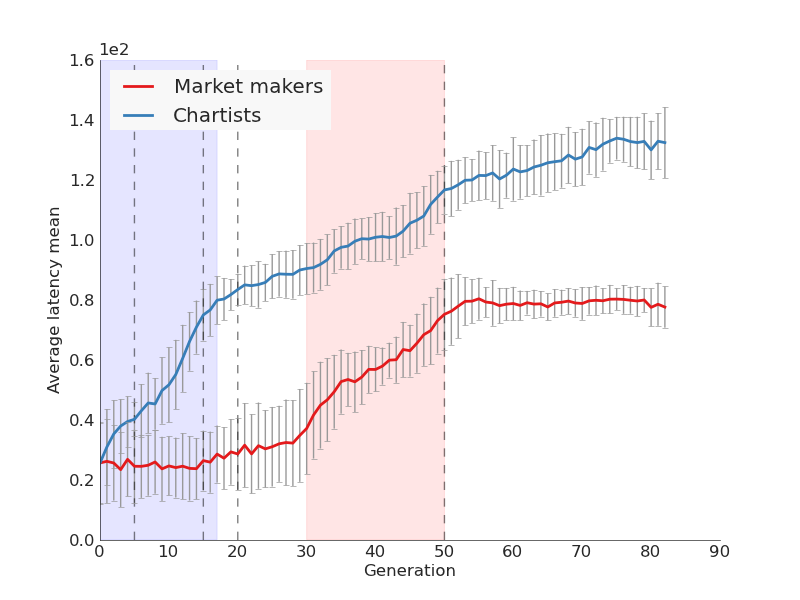
\includegraphics[width=0.5\textwidth]{82_generation_plots/d11/latpars_mu.png}}
	\subcaptionbox{Evolution of \ssmmlatencys{} and \sclatencys}
	[0.49\linewidth]{\includegraphics[width=0.5\textwidth]{82_generation_plots/d11/latpars_s.png}}
	\subcaptionbox{Evolution of \scnAgents}
	[0.49\linewidth]{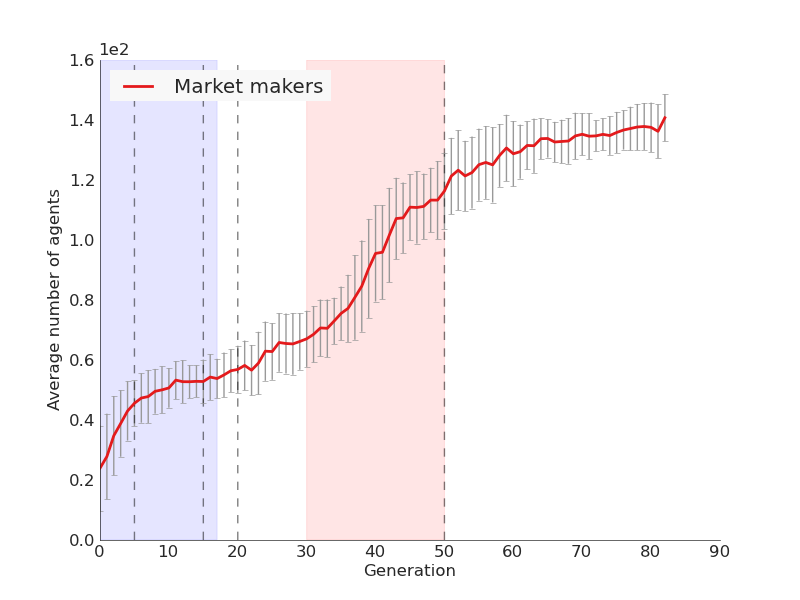
\includegraphics[width=0.5\textwidth]{82_generation_plots/d11/nAgents.png}}
	\caption{Evolution of the model parameters in experiment \deleven}
	\label{fig:d11_evolution_parameters}
\end{figure}

\begin{figure}
	%issue 15
	\centering
	\subcaptionbox{Evolution of \roundstable}
	[0.49\linewidth]{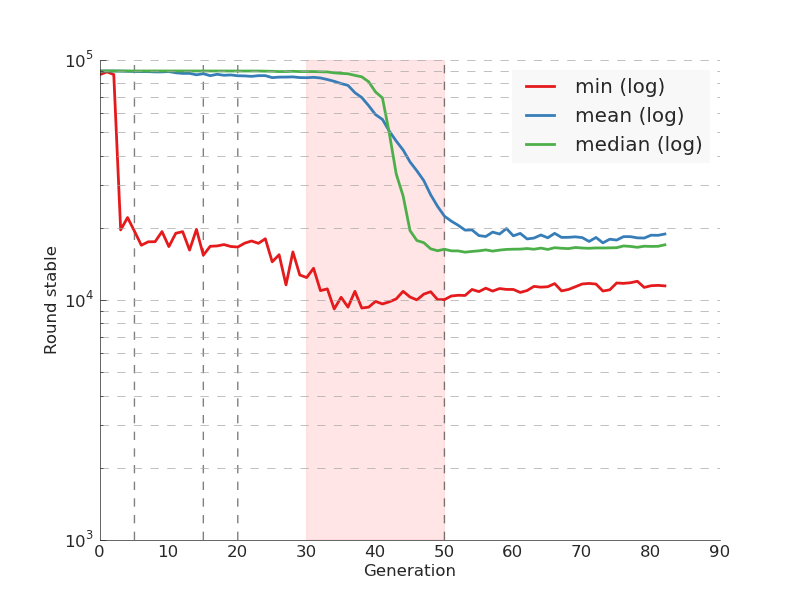
\includegraphics[width=0.5\textwidth]{82_generation_plots/d11/round_stable.png}}
	\subcaptionbox{Evolution of \timetoreachnewfundamental}
	[0.49\linewidth]{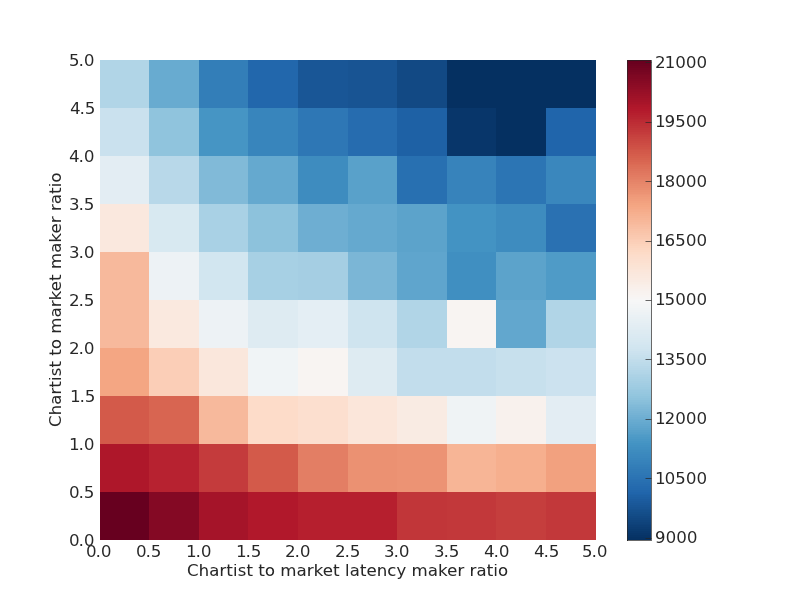
\includegraphics[width=0.5\textwidth]{82_generation_plots/d11/time_to_reach_new_fundamental.png}}
	\subcaptionbox{Evolution of \stdev}
	[0.49\linewidth]{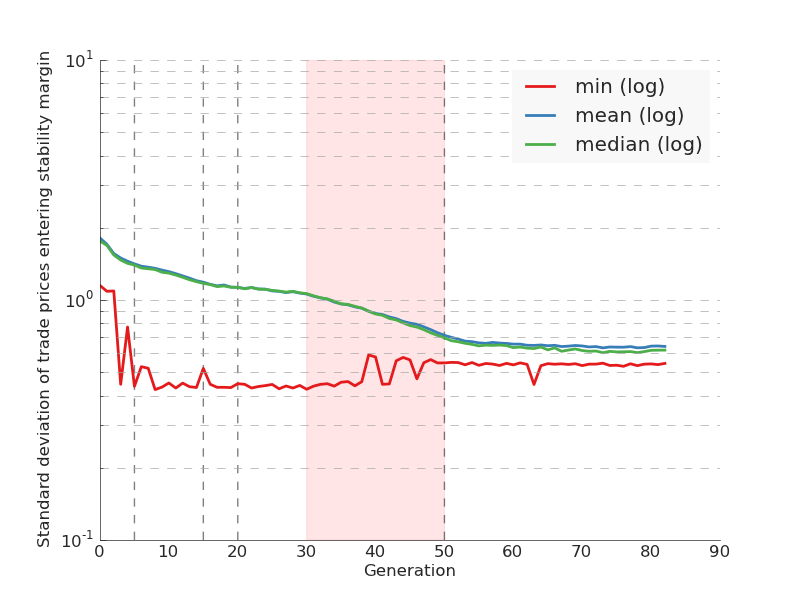
\includegraphics[width=0.5\textwidth]{82_generation_plots/d11/stdev.png}}
	\subcaptionbox{Evolution of \overshoot}
	[0.49\linewidth]{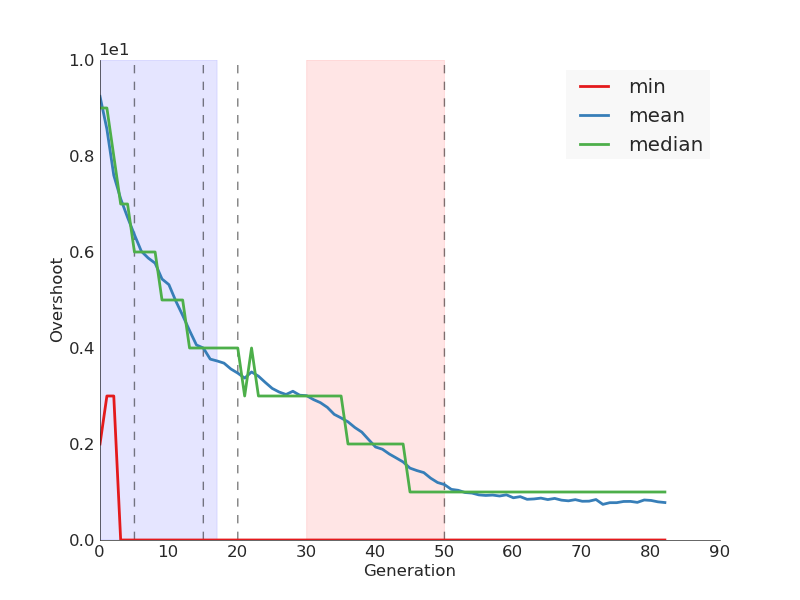
\includegraphics[width=0.5\textwidth]{82_generation_plots/d11/overshoot.png}}
	\caption{Evolution of the four fitness measures in experiment \deleven}
	\label{fig:d11_evolution_fitness}
\end{figure}

\begin{figure}
	%issue 15
	\centering
	\subcaptionbox{Correlation between \sclatencymu{} and \overshoot}
	[0.49\linewidth]{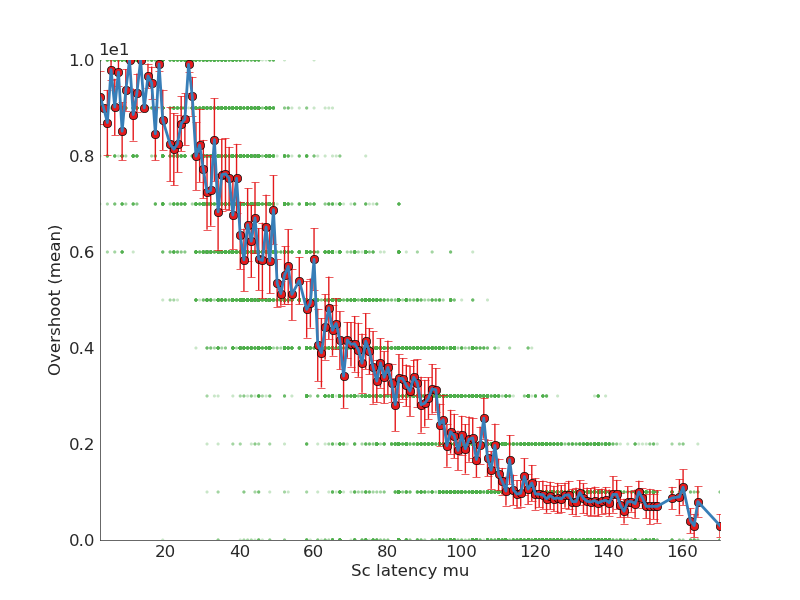
\includegraphics[width=0.5\textwidth]{101_pars_vs_fits/d11/sc_latency_mu__vs__overshoot(mean)_scatter.png}}
	\subcaptionbox{Correlation between \sclatencymu{} and \roundstable}
	[0.49\linewidth]{\includegraphics[width=0.5\textwidth]{101_pars_vs_fits/d11/sc_latency_mu__vs__round_stable(mean)_scatter.png}}
	\subcaptionbox{Correlation between \sclatencymu{} and \stdev}
	[0.49\linewidth]{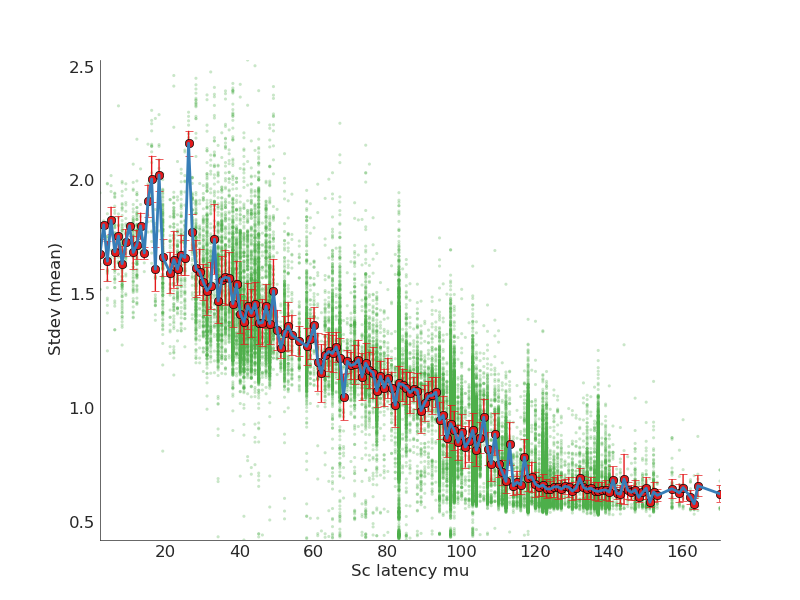
\includegraphics[width=0.5\textwidth]{101_pars_vs_fits/d11/sc_latency_mu__vs__stdev(mean)_scatter.png}}
	\subcaptionbox{Correlation between \sclatencymu{} and \timetoreachnewfundamental}
	[0.49\linewidth]{\includegraphics[width=0.5\textwidth]{101_pars_vs_fits/d11/sc_latency_mu__vs__time_to_reach_new_fundamental(mean)_scatter.png}}
	
	\caption{Correlation between \sclatencymu and the four fitness measures in experiment \deleven}
	\label{fig:d11_parvfit_sclatencymu}
\end{figure}

\begin{figure}
	%issue 15
	\centering
	\subcaptionbox{Correlation between \ssmmlatencymu{} and \overshoot}
	[0.49\linewidth]{\includegraphics[width=0.5\textwidth]{101_pars_vs_fits/d11/ssmm_latency_mu__vs__overshoot(mean)_scatter.png}}
	\subcaptionbox{Correlation between \ssmmlatencymu{} and \roundstable}
	[0.49\linewidth]{\includegraphics[width=0.5\textwidth]{101_pars_vs_fits/d11/ssmm_latency_mu__vs__round_stable(mean)_scatter.png}}
	\subcaptionbox{Correlation between \ssmmlatencymu{} and \stdev}
	[0.49\linewidth]{\includegraphics[width=0.5\textwidth]{101_pars_vs_fits/d11/ssmm_latency_mu__vs__stdev(mean)_scatter.png}}
	\subcaptionbox{Correlation between \ssmmlatencymu{} and \timetoreachnewfundamental}
	[0.49\linewidth]{\includegraphics[width=0.5\textwidth]{101_pars_vs_fits/d11/ssmm_latency_mu__vs__time_to_reach_new_fundamental(mean)_scatter.png}}
	
	\caption{Correlation between \sclatencymu{} and the four fitness measures in experiment \deleven}
	\label{fig:d11_parvfit_ssmmlatencymu}
\end{figure}


\begin{figure}
	%issue 15
	\centering
	\subcaptionbox{Correlation between \scnAgents{} and \overshoot}
	[0.49\linewidth]{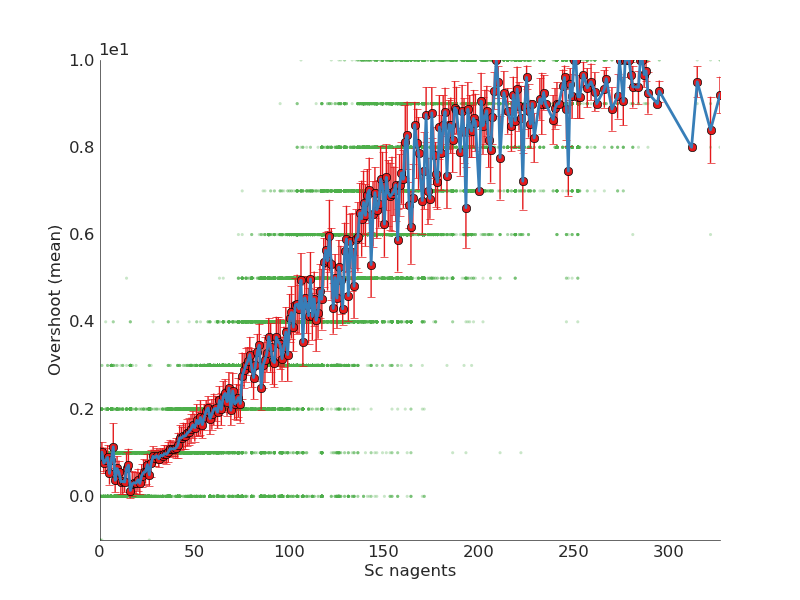
\includegraphics[width=0.5\textwidth]{101_pars_vs_fits/d11/sc_nAgents__vs__overshoot(mean)_scatter.png}}
	\subcaptionbox{Correlation between \scnAgents{} and \roundstable}
	[0.49\linewidth]{\includegraphics[width=0.5\textwidth]{101_pars_vs_fits/d11/sc_nAgents__vs__round_stable(mean)_scatter.png}}
	\subcaptionbox{Correlation between \scnAgents{} and \stdev}
	[0.49\linewidth]{\includegraphics[width=0.5\textwidth]{101_pars_vs_fits/d11/sc_nAgents__vs__stdev(mean)_scatter.png}}
	\subcaptionbox{Correlation between \scnAgents{} and \timetoreachnewfundamental}
	[0.49\linewidth]{\includegraphics[width=0.5\textwidth]{101_pars_vs_fits/d11/sc_nAgents__vs__time_to_reach_new_fundamental(mean)_scatter.png}}
	
	\caption{Correlation between \ssmmnAgents{} and the four fitness measures in experiment \deleven}
	\label{fig:d11_parvfit_scAgents}
\end{figure}
\end{comment}


\section{Hall of fame}\label{section:hall_of_fame}
